%!TEX TS-program = xelatex
%!TEX root = ../../maxwell2018thesis.tex

\chapter[Discussion and Future Work]{Discussion and Future Work}\label{chap:conclusions}
The final chapter of this thesis summarises and discusses the results reported in this thesis. In particular, we emphasise the impact of our findings on~\gls{acr:ir} and~\gls{acr:iir} research, as well as outlining several potential future research directions. We then conclude the thesis with some final remarks.

\section{Thesis Summary}\label{sec:conclusions:summary}
In this thesis, we examined how stopping behaviours vary under different search contexts. In particular, we conducted and reported on two user studies under the domain of news search, examining how~\raisebox{-.2\height}{\includegraphics[height=5mm]{figures/ch2-point1.pdf}} result summary lengths and~\raisebox{-.2\height}{\includegraphics[height=5mm]{figures/ch2-point2.pdf}} a variation of search tasks, goals and retrieval systems affected search behaviours. A total of eight different interfaces and conditions were used to examine how behaviours vary. Table~\ref{tbl:conclusion_cond_interface_summary} presents a summary of the aforementioned interfaces and conditions, concerning the length of result summaries, the systems and tasks used.

\begin{table}[t!]
    \caption[Summary of experimental interfaces and conditions]{A summary table of the different experimental interfaces and conditions that were trialled. These are based upon the work reported in Chapters~\ref{chap:snippets} and~\ref{chap:diversity}. In total, eight different experimental interfaces and conditioned were employed, considering different result summary lengths, systems and tasks.}
    \label{tbl:conclusion_cond_interface_summary}
    \renewcommand{\arraystretch}{1.8}
    \begin{center}
    \begin{tabulary}{\textwidth}{L{0.4cm}@{\CS}L{3.2cm}@{\CS}D{3.51cm}@{\CS}D{3.51cm}@{\CS}D{3.51cm}@{\CS}}
        & & \lbluecell \textbf{Summary Length} & \lbluecell \textbf{System} & \lbluecell \textbf{Task} \\
        
        \RS \multirow{4}{*}{\rotatebox{90}{\hspace*{-4mm}\textbf{Chapter~\ref{chap:snippets}}}} & \lbluecell\textbf{T0} & \cell \small{Title only} & \cell \small{\blueboxbold{ND} (Non Div.)} & \cell \small{\darkblueboxbold{AD} (Ad-hoc)}\\
        \RS & \lbluecell\textbf{T1} & \cell \small{Title + 1 snippet} & \cell \small{\blueboxbold{ND} (Non Div.)} & \cell \small{\darkblueboxbold{AD} (Ad-hoc)}\\
        \RS & \lbluecell\textbf{T2} & \cell \small{Title + 2 snippets} & \cell \small{\blueboxbold{ND} (Non Div.)} & \cell \small{\darkblueboxbold{AD} (Ad-hoc)}\\
        \RS & \lbluecell\textbf{T4} & \cell \small{Title + 4 snippets} & \cell \small{\blueboxbold{ND} (Non Div.)} & \cell \small{\darkblueboxbold{AD} (Ad-hoc)}\\
        
        \RS\RS\RS \multirow{4}{*}{\rotatebox{90}{\hspace*{-4mm}\textbf{Chapter~\ref{chap:diversity}}}} & \lbluecell\textbf{D-AS} & \cell \small{Title + 2 snippets} & \cell \small{\blueboxbold{D} (Div.)} & \cell \small{\darkblueboxbold{AS} (Aspectual)}\\
        \RS & \lbluecell\textbf{ND-AS} & \cell \small{Title + 2 snippets} & \cell \small{\blueboxbold{ND} (Non Div.)} & \cell \small{\darkblueboxbold{AS} (Aspectual)}\\
        \RS & \lbluecell\textbf{D-AD} & \cell \small{Title + 2 snippets} & \cell \small{\blueboxbold{D} (Div.)} & \cell \small{\darkblueboxbold{AD} (Ad-hoc)}\\
        \RS & \lbluecell\textbf{ND-AD} & \cell \small{Title + 2 snippets} & \cell \small{\blueboxbold{ND} (Non Div.)} & \cell \small{\darkblueboxbold{AD} (Ad-hoc)}\\
        
    \end{tabulary}
    \end{center}
\end{table}

From the first user study reported in Chapter~\ref{chap:snippets}, results showed that as result summary lengths increased (from \blueboxbold{T0}$\rightarrow$\blueboxbold{T4}), searchers became more confident in the decisions they took pertaining to the relevance of documents encountered. However, this was not reflected empirically; their accuracy in identifying relevant content did not improve with longer result summaries. In terms of stopping behaviours, a downward trend was observed. As the length of result summaries increased, subjects examined to shallower depths per query -- an intuitive result, given the increased examination times required for longer summaries.

Considering variations of tasks, goals and systems as reported in Chapter~\ref{chap:diversity}, we found that when using diversified system \blueboxbold{D} (i.e. BM25 and XQuAD~\citep{santos2010query_reformulations_diversification}), subjects issued more queries and stopped at comparatively shallow depths per query. This was in comparison to non-diversified system (i.e. BM25 baseline) \blueboxbold{ND}, where subjects reported feeling less confident with their decisions. Despite the significant differences we observed between how the two systems performed, few significant differences were reported in empirical evidence concerning changes in searcher behaviours. Most subjects also reported difficulties in discerning notable differences between the two systems.

Interaction data from these user studies were then used to ground an extensive set of simulations of interaction. These simulations were designed to test a total of twelve individual stopping strategies, derived from a variety of stopping heuristics\footnote{Stopping heuristics for example considered a searcher's tolerance to non-relevance, or their \emph{frustration} with observing non-relevant content~\citep{kraft1979stopping_rules}.} and~\gls{acr:ir} measures as defined in the literature. Their cataloguing and subsequent operationalisation into stopping strategies provided an answer to \darkblueboxbold{HL-RQ2}. Testing overall performance and how closely the simulations matched up to real-world searcher behaviours across the eight experimental interfaces and conditions, we could then provide answers to both \darkblueboxbold{HL-RQ3a} and \darkblueboxbold{HL-RQ3b}. The simulations were based upon the~\glsfirst{acr:csm}, an updated, high-level conceptual model of the search process. By incorporating a new~\gls{acr:serp} level stopping decision point into the~\gls{acr:csm}, complete with subsequent empirical evaluation (as presented in Chapter~\ref{chap:serp}), we could then provide an answer to \darkblueboxbold{HL-RQ1}.

Results show that when enabled, the new~\gls{acr:serp} stopping decision point led to significant improvements over the baseline implementation, with consistent improvements in overall performance (measured in~\gls{acr:cg}) reported across a range of experimental conditions, interfaces and stopping strategies. In consideration of approximating real-world searcher stopping behaviours, improvements are also present -- these however were not significantly different. Overall, these results provide compelling evidence for \darkblueboxbold{HL-RQ1}, and also demonstrate a promising direction for future research in developing our understanding of the search process.

With respect to our simulated analyses of individual stopping strategies, we found several stopping strategies offered the highest overall levels of~\gls{acr:cg} and good approximations with actual searcher stopping behaviours. For example, as result summary lengths increased, we found that \blueboxbold{SS11-COMB} consistently offered the best performance, with both \blueboxbold{SS1-FIX} and \blueboxbold{SS4-SAT} offering the best real-world searcher approximations. \blueboxbold{SS5-COMB} also offered the best overall levels of~\gls{acr:cg} across the second user study, with \blueboxbold{SS1-FIX} again offering the best levels of performance across condition \dualbluebox{ND}{AD}. In terms of approximations, \blueboxbold{SS1-FIX} and \blueboxbold{SS10-RELTIME} yielded the lowest MSE values. However, despite these strategies performing well, no one strategy clearly emerged as offering significantly improved levels of performance or approximations. However, several more complex stopping strategies such as \blueboxbold{SS6-DT} and \blueboxbold{SS7-DKL} consistently offered poorer performance and approximations. This is a common theme in our results: simple and combination-based stopping strategies generally performed the best. This includes the fixed-depth stopping strategy, \blueboxbold{SS1-FIX}, which, counter to our intuition, consistently performed well.

\section{Discussion}\label{sec:conclusions:discussion}
From the analysis of our simulations of interaction, a number of interesting areas of discussion became apparent. In this section, we discuss our findings with an emphasis on examining the stopping strategies that were trialled. In particular, our discussion is guided by our four high-level research questions. We repeat these below.

\begin{itemize}
    \item{\darkblueboxbold{HL-RQ1} How can we improve searcher models to incorporate different stopping decision points?}
    \item{\darkblueboxbold{HL-RQ2} Given the stopping heuristics defined in the literature, how can we encode these heuristics into a series of operationalised, programmable stopping strategies that can be subsequently incorporated into the searcher model and be evaluated?}
    \item{\darkblueboxbold{HL-RQ3a} Given the aforementioned operationalised stopping strategies, how well does each one perform?}
    \item{\darkblueboxbold{HL-RQ3b} How closely do the operationalised stopping strategies compare to the actual stopping behaviours of real-world searchers?}
\end{itemize}

With these research questions pertaining to the simulations of interaction (along with the implemented stopping strategies), in-depth discussion of our user studies can be found in Sections~\ref{chap:snippets:user:discussion} on page~\pageref{chap:snippets:user:discussion} and~\ref{sec:diversity:users:discussion} on page~\pageref{sec:diversity:users:discussion}. However, we do briefly touch on summarising statements relating to searcher behaviours in Section~\ref{sec:conclusions:discussion:behaviours}.

\subsection{Searcher Models and Realism}\label{sec:conclusions:discussion:realism}
\todo{TO ADD IN. THIS IS POSITIVE.}

- inclusion of new stopping decision point helps.
- improves the realism of the experiments.

- what about other stopping strategies?
    - reason to believe that they would offer improvements, too.

- probabilities were similar across each of the different SERP decision point interface/conditions.

- say that we focus on the Perfect approach. Of course we do, we want to demonstrate improvements.
- average also helps. but maybe more runs were required. see Section~\ref{sec:conclusions:discussion:simulations}

\subsection{Stopping Strategy Operationalisation}\label{sec:conclusions:discussion:strategies}
In general, findings across all interfaces and conditions trialled demonstrated that simple stopping strategies tended to yield better performance, and matched better with real-world searcher stopping behaviours. Strategies \blueboxbold{SS2-NT}, \blueboxbold{SS3-NC}, \blueboxbold{SS4-SAT}, \blueboxbold{SS9-TIME} and \blueboxbold{SS10-RELTIME} all for example performed and approximated well. We consider these simple in the sense that the stopping criterion that they each encoded was straightforward to implement and subsequently measure, considering aspects such as the number of non-relevant documents encountered, or the elapsed time spent searching since query issuance.

In contrast, findings also demonstrated that the more complex stopping strategies tended to perform worse. They consistently offered poorer performance and approximations. Complexity was again denoted by the criterion/criteria that were considered by each strategy, with more complex computations required in order to determine when the simulated searcher should stop. Given these general findings, \emph{why did the more complex stopping strategies perform and approximate worse on average?} This section of the discussion focuses primarily on this question, considering the difference-based strategies \blueboxbold{SS6-DT} and \blueboxbold{SS7-DKL}, the~\gls{acr:ift}-based strategy \blueboxbold{SS8-IFT}, and the~\gls{acr:rbp}-based strategy \blueboxbold{SS12-RBP}.

\blueboxheader{Difference Stopping Strategies}
Considering \blueboxbold{SS6-DT} and \blueboxbold{SS7-DKL}, we hypothesise that the performance of issued queries may be having an effect on the way in which these strategies perform. In other words, the stopping strategies \emph{may not be very robust} to varying levels of query performance. Recall that for our \emph{what-if} performance runs, we employed an interleaved querying strategy, \blueboxbold{QS13}.\footnote{Refer to Section~\ref{sec:method:simulation:grounding:querying} on page~\pageref{sec:method:simulation:grounding:querying} for additional information on how the querying strategy was implemented.} With this strategy, single term and three term queries were interleaved together. From empirical evidence, it was shown that single term queries offered poor performance (in terms of $P@k$) when compared to three term queries -- single term queries offered higher levels of diversity compared to the three term queries.\footnote{For example, consider the queries \texttt{`piracy'} and \texttt{`piracy china sea'}. The first single term query returned a majority of documents pertaining to software piracy, along with piracy at sea. In contrast, the three term query returned a majority of its matched documents to instances of piracy on the South China Sea, relevant to the~\gls{acr:trec} piracy topic.} As such, using a fixed threshold across queries of varying performance would not necessarily make sense. A low threshold for \blueboxbold{SS6-DT} and \blueboxbold{SS7-DKL} would mean that searchers would stop too early for single term queries, and examine too deep for three term queries. A higher threshold would mean that searchers would browse too deep for single and three term queries. This means that a low threshold for example would be too stringent for single term queries, and suggests that poor levels of gain would be accumulated.

\begin{figure}[t!]
    \centering
    \resizebox{1\hsize}{!}{
    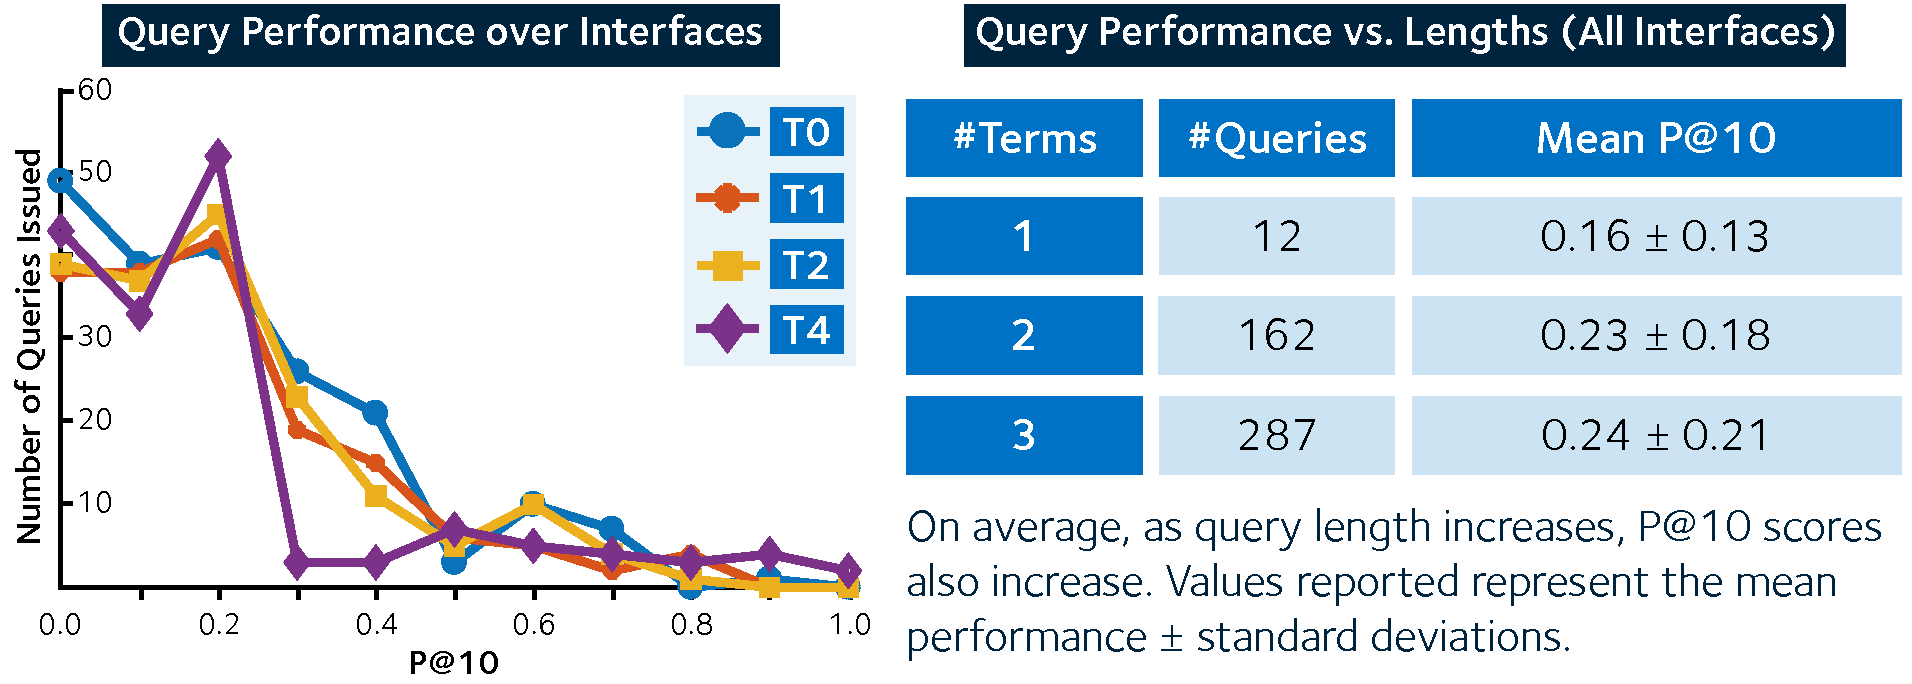
\includegraphics{figures/ch10-queryperf.pdf}}
    \caption[Query performance by real-world subjects]{Plot demonstrating the performance of queries (\genericblack{P@10}) across the four experimental interfaces trialled in the user study we report on in Chapter~\ref{chap:snippets}. On the right, a table highlights the varying levels of performance (averaged over all four experimental interfaces) in relation to query term lengths. As query term length increases, so too does the mean P@10 score. Similar findings were observed for the study reported in Chapter~\ref{chap:diversity}.}
    \label{fig:query_performance_ch7}
\end{figure}

As such, we hypothesise that for stopping strategies based upon the difference-based heuristic, thresholds should likely be query specific -- perhaps dependent upon the length of the query issued. Given queries issued by the real-world subjects in Chapter~\ref{chap:snippets}, we also observed a large variation in performance for the queries that were issued. We report this in Figure~\ref{fig:query_performance_ch7}, with a plot showing the number of queries issued across each of the four interfaces, plotted against the performance of the queries. A table also provides evidence to back our hypothesis, showing that as the number of terms in the queries increased, so too did the mean level of query performance. Similar findings were observed in the user study reported in Chapter~\ref{chap:diversity}.

\blueboxheader{\gls{acr:ift} Stopping Strategy}
Next, we consider the poor performance and approximations afforded by \blueboxbold{SS8-IFT}. Evidence has shown that~\gls{acr:ift} has been proven to be good at predicting search behaviours, with examples of recent studies demonstrating this by~\cite{ong2017scent_behaviour} and~\cite{azzopardi2018cwl}. In Section~\ref{sec:diversity:users:results:ift} on page~\pageref{sec:diversity:users:results:ift}, we demonstrated that our~\gls{acr:ift}-based hypotheses matched up closely with empirical evidence. So, why did \blueboxbold{SS8-IFT} then proceed to consistently offer poorer performance and approximations when compared to more simplistic stopping strategies? We hypothesise that this comparative lack of performance can be attributed to how the \emph{rate of gain} was operationalised, which serves as the stopping criterion for \blueboxbold{SS8-IFT}. This is an inherently difficult value to compute, with limitations relating to the rate of gain considered from two angles:

\begin{itemize}
    \item[\raisebox{-.2\height}{\includegraphics[height=5mm]{figures/ch2-point1.pdf}}]{the \emph{per-topic} rate of gain; and}
    \item[\raisebox{-.2\height}{\includegraphics[height=5mm]{figures/ch2-point2.pdf}}]{\emph{how the rate of gain is estimated} by searchers in the first instance.}
\end{itemize}

\begin{figure}[t!]
    \centering
    \resizebox{1\hsize}{!}{
    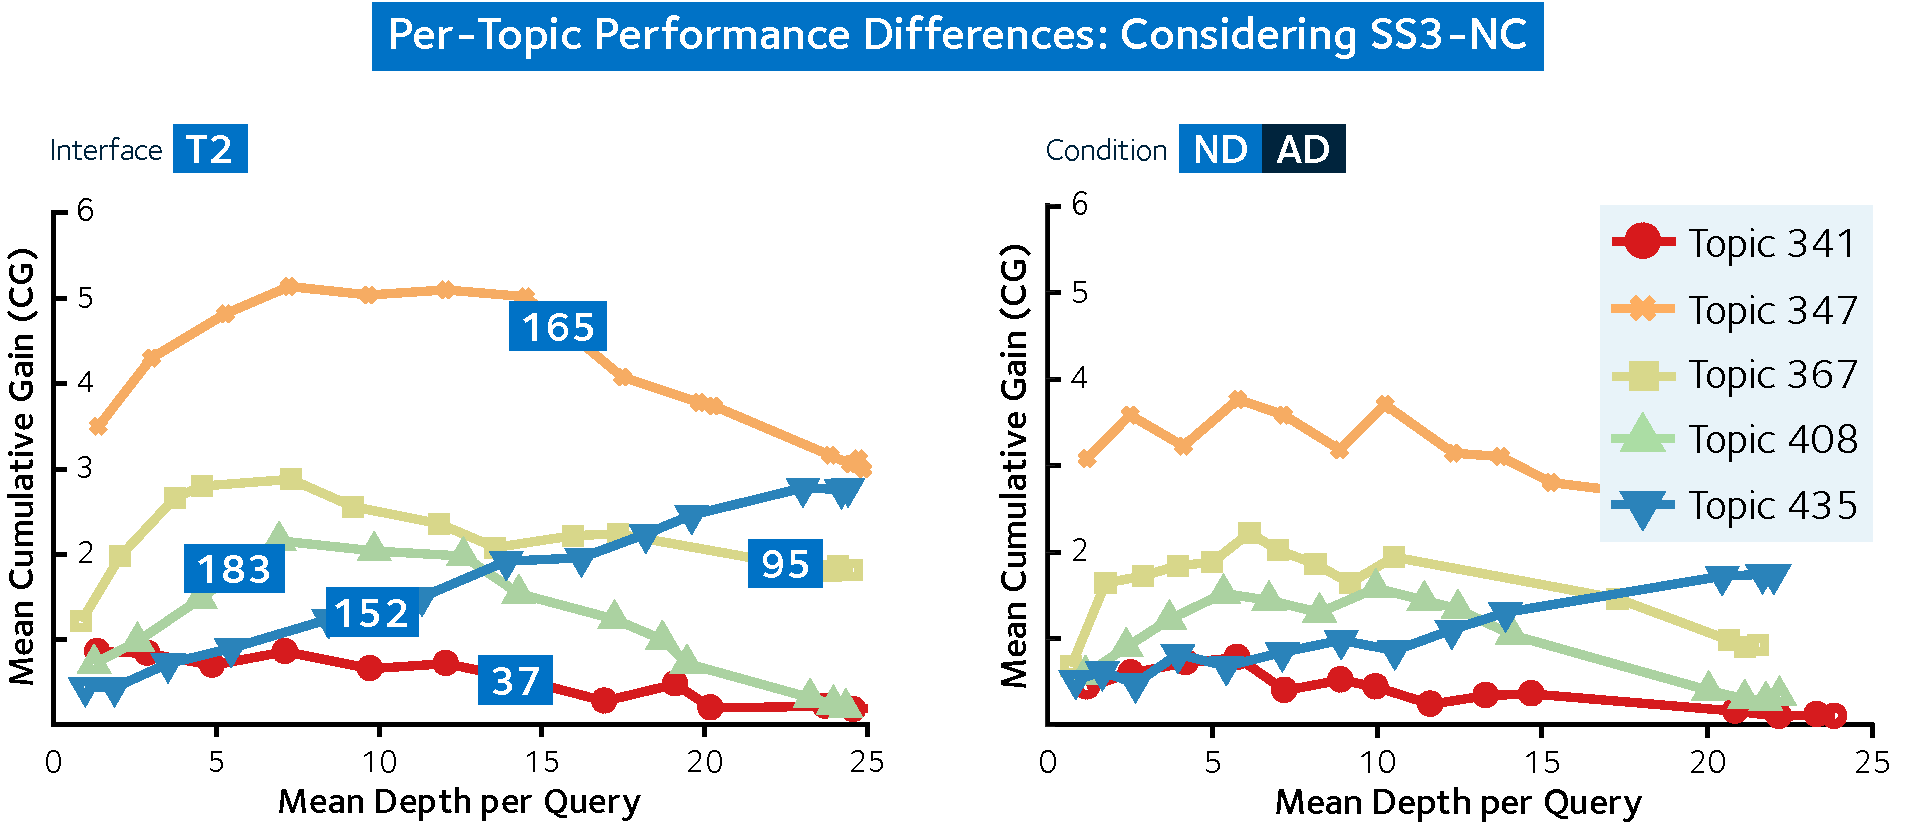
\includegraphics{figures/ch10-per_topic.pdf}}
    \caption[Per-topic performance variation example]{Plots demonstrating the wide per-topic variance over the \emph{what-if} performance simulations. On the left, performance over interface \blueboxbold{T2} is shown – \dualbluebox{ND}{AD} is shown on the right. Stopping strategy \blueboxbold{SS3-NC} is used for this demonstration. Similar observations could be observed across other interfaces, conditions and stopping strategies. Also \blueboxbold{highlighted} on the left plot is the number of~\gls{acr:trec} relevant documents for each topic. Note the general performance improvement as the number of~\gls{acr:trec} relevant documents increases for a topic.}
    \label{fig:per_topic_differences}
\end{figure}

Considering point~\raisebox{-.2\height}{\includegraphics[height=5mm]{figures/ch2-point1.pdf}} first, we note that the same gain stopping threshold values were trialled over all five topics in the reported simulations of interaction. Table~\ref{tbl:ch6_topic_rels} on page~\pageref{tbl:ch6_topic_rels} demonstrated that the number of~\gls{acr:trec} relevant documents for each of the five topics varies considerably. As such, one would expect that the computed rate of gain would also vary considerably on a per-topic basis. This way, expectations of gain can be kept in check -- a rate of gain threshold computed over a performant~\gls{acr:trec} topic with many relevant documents would perform much worse under a topic that is much harder to find relevant documents for (i.e. a comparatively smaller number of~\gls{acr:trec} relevant documents). This varying number of relevant documents over topics (amongst other factors, such as the retrieval system used) is illustrated in Figure~\ref{fig:per_topic_differences}. Using interface \blueboxbold{T2} (left) and condition \dualbluebox{ND}{AD} (right) over \blueboxbold{SS3-NC}, the two plots in the figure illustrate the variation in performance across the five topics trialled. We also note a general trend of higher performance for a topic in the plots if a greater number of~\gls{acr:trec} relevant documents are present.

We also consider how the rate of gain is computed, as per point~\raisebox{-.2\height}{\includegraphics[height=5mm]{figures/ch2-point2.pdf}}. \emph{How do searchers estimate a rate of gain threshold?} This is a difficult question to answer, with further study required to address this. However, one would be pressed to believe that from an initial impression of a~\gls{acr:serp}, a searcher would undertake a series of computations in their head to reach an estimation for a rate of gain threshold value. It is much easier to believe that searchers instead would employ a simpler stopping criterion in in this instance, such as \emph{stopping after observing $k$ non-relevant result summaries} (i.e. the frustration-based heuristic). This can be simplified with an individual throwing a ball in the air. For example, it would be easier to believe that the ball thrower would think of how to catch the ball in relation to how it is falling through the air, with feedback from their visual and proprioception systems. This is opposed to believing that the ball thrower can catch the ball via calculating the physics behind the ball falling, and working out the optimal point in space at which to catch it.


\blueboxheader{\gls{acr:rbp} Stopping Strategy}
What???

\blueboxheader{More Performant Stopping Strategies}
What???


\subsection{Searcher Behaviours}\label{sec:conclusions:discussion:behaviours}

\subsection{Simulations of Interaction}\label{sec:conclusions:discussion:simulations}

\section{Future Research Directions}\label{sec:conclusions:future}

\subsection{Improving Simulation Realism}\label{sec:conclusions:future:improving}

\subsection{Stopping Heuristics and Strategies}\label{sec:conclusions:future:stopping}

\subsection{Simulation Trials and Topics}\label{sec:conclusions:future:running}

\subsection{Individual Searcher Stopping Behaviours}

\section{Final Remarks}\label{sec:conclusions:remarks}